% Teilauswertung 4

\section{Lock-In Verstärker}
\label{sec:lockin}

\paragraph{a)}\textbf{Lock-In Verstärker als Filter}\\
Im folgenden Teil wollen wir die den Lock-In Verstärker als Filter verwenden und die Ausgangsmesswerte der Sinus, Rechteck und Dreieckschwingung interpretieren.

Die Messungen haben folgende Tabelle ergeben:
\begin{center}
    \begin{tabular}{l | c c c c c c c}
        f/kHz               & 1 & 3 & 5 & 7 & 9 & 11 & 13 \\
        \hline
        $U_{eff,Sinus}$/V     & 0,7072 & 0.0000 & 0.0000 & 0.0000 & 0.0000 & 0.0000 & 0.0000 \\
        $U_{eff,Rechteck}$/V  & 0,9003 & 0.3000 & 0.1800 & 0.1285 & 0.1000 & 0.0817 & 0.0692 \\
        $U_{eff,Dreieck}$/V   & 0,5733 & 0.0636 & 0.0229 & 0.0117 & 0.0070 & 0.0047 & 0.0034 \\
    \end{tabular}
    \captionof{table}{Messung Lock-In Verstärker als Filter bei unterschiedlichen Signalen}
    \label{tab:lockinFilter}
\end{center}
In der Tabelle \ref{tab:lockinFilter} ist schon angedeutet, dass sich bei den gemessenen Spannungswerte um die Effektivspannungswerte der jeweiligen Schwingung handelt. Wie schon in Kapitel \ref{sec:mittelungAndTrafo}a) kann man die Effektivspannungswerte in die Werte der Fourierentwicklungskoeffizienten umrechnen, indem man die Messwerte mit dem Faktor $\sqrt{2}$ multipliziert. Zum Vergleich mit der Theorie wird zugleich die errechneten Werte aus Tabelle \ref{tab:fourierkoeff} verwendet. Damit erhält man:
\begin{center}
    \begin{tabular}{c | c c | c c | c c}
        \textbf{Frequenz} & \multicolumn{2}{c|}{\textbf{Sinus}} & \multicolumn{2}{c|}{\textbf{Rechteck}} & \multicolumn{2}{c}{\textbf{Dreieck}}\\
        $f$/kHz & $U_{Mess}$/V & $U_{Theo}$/V & $U_{Mess}$/V & $U_{Theo}$/V & $U_{Mess}$/V & $U_{Theo}$/V\\
        \hline
         1 &  1.0001 &  1.0000 & 1.2732 & 1.2732 & 0.8107 & 0.8106 \\
         3 &  0.0000 &  0.0000 & 0.4243 & 0.4244 & 0.0899 & 0.0900 \\
         5 &  0.0000 &  0.0000 & 0.2546 & 0.2546 & 0.0324 & 0.0324 \\
         7 &  0.0000 &  0.0000 & 0.1817 & 0.1819 & 0.0165 & 0.0165 \\
         9 &  0.0000 &  0.0000 & 0.1414 & 0.1415 & 0.0099 & 0.0100 \\
        11 &  0.0000 &  0.0000 & 0.1155 & 0.1157 & 0.0066 & 0.0067 \\
        13 &  0.0000 &  0.0000 & 0.0979 & 0.0979 & 0.0048 & 0.0048 \\
    \end{tabular}
    \captionof{table}{Vergleich Theorie und Praxis bei der Messung mit Lock-In Verstärker}
    \label{tab:lockinFourierkoeff}
\end{center} 
In Tabelle \ref{tab:lockinFourierkoeff} sieht man ganz deutlich wie präzise die Messung mit einem Lock-In Verstärkers ist. In der Berechnung hat man dabei bewusst auf die Fehlerrechnung verzichtet, da diese Fehler nur in der Größenordnung von $\pm 0,0001$V liegt. Im Vergleich zu Tabelle \ref{tab:fourierkoeff} hat der Lock-In Verstärker aber eine deutlich höhere Präzession der Messung, da bei der Messung vor allem bei Frequenzen von 1kHz eine Abweichung von ungefähr 0,002V zu verzeichnen war.
\newpage
\paragraph{b)}\textbf{Bandbreite des Lock-In Verstärkers}\\
Als Nächstes wird die Zeitkonstante und die damit verbundene Ordnung des Filters des Lock-In Verstärkers bestimmt. Dafür wurde an dem Lock-In Verstärker eine Sinusschwingung mit einer Frequenz von 1kHz und eine Amplitude von 100mV angelegt. Am Lock-In Verstärker wurde die Flankensteilheit $\Delta$ des eingebauten Tiefpassfilters von 6dB auf 18dB verändert und eine Zeitkonstante $\tau$ von 30ms eingestellt. Um die Zeitkonstante und Ordnung zu bestimmen wird eine Kurve durch die aufgenommene Messreihe gefittet. Die Form der Kurve wurde uns im Praktikum zur Verfügung gestellt worden und ist speziell für den Lock-In Verstärker SR830 DSP. Die Kurve hat dann die Gleichung:
\begin{gather}
    A_{\tau,n}(f) = \left[1 + (2\pi\tau(f-f_0))^2\right]^{-\frac{n}{2}}
\end{gather}
Diese Gleichung beschreibt hierbei die Filterantwort des Lock-In Verstärkers, wobei \newline $n$ die Ordnung, $\tau$ die Zeitkonstante des Filters und $A$ die normierte Amplitude ist. Die Frequenz $f_0$ ist die eingestellte Frequenz der Sinusschwingung und liegt bei 1kHz. Die Normierung erfolgt über den maximalen Wert der Effektivspannung, welcher bei den Frequenz $f_0$ liegt. Durch die Normierung muss die Umwandlung von Effektivspannung in tatsächliche Spannung nicht berücksichtigt werden. Es wurde wieder auf eine Fehlerrechnung verzichtet, da die Fehler zu klein sind. Der Fit liefert dann folgende Parameter:
\begin{center}
    \begin{tabular}{c | c c}
        $\Delta$/dB & $\tau$/ms & $n$\\
        \hline
        6 & 27.35 & 1.06 \\
        18 & 30.16 & 3.00 \\
    \end{tabular}
    \captionof{table}{Ergebnis gefittete Parameter für $\tau$ und $n$}
    \label{tab:fitPara}
\end{center}
In Abbildung \ref{image:6dB} und \ref{image:18dB} sind jeweils die Fit für die jeweilige Messreihe dargestellt. Beim Vergleich der gefitteten Werte der Zeitkonstante $\tau$ mit dem tatsächlichen eingestellten Wert von 30ms zeigt, dass die Messung des Lock-In Verstärkers eine genaue Bestimmung der Zeitkonstante $\tau$ zulässt. Ein guter Indikator ist hierbei die Ordnung $n$, da die genau Zeitkonstante $\tau$ dann erzielt wurden als $n$ ganzzahlig war.

Auch ist zu erkennen, dass durch eine Verdreifachung der Flankensteilheit $\Delta$ auch die Ordnung $n$ des Filters sich verdreifacht hat. Gut zu erkennen ist dies auch in Abbildung \ref{image:All}, in der die gefittete Kurve für $\Delta=18$dB viel schmäler ist als die gefittete Kurve für $\Delta=6$dB.
\newpage
\begin{center}
    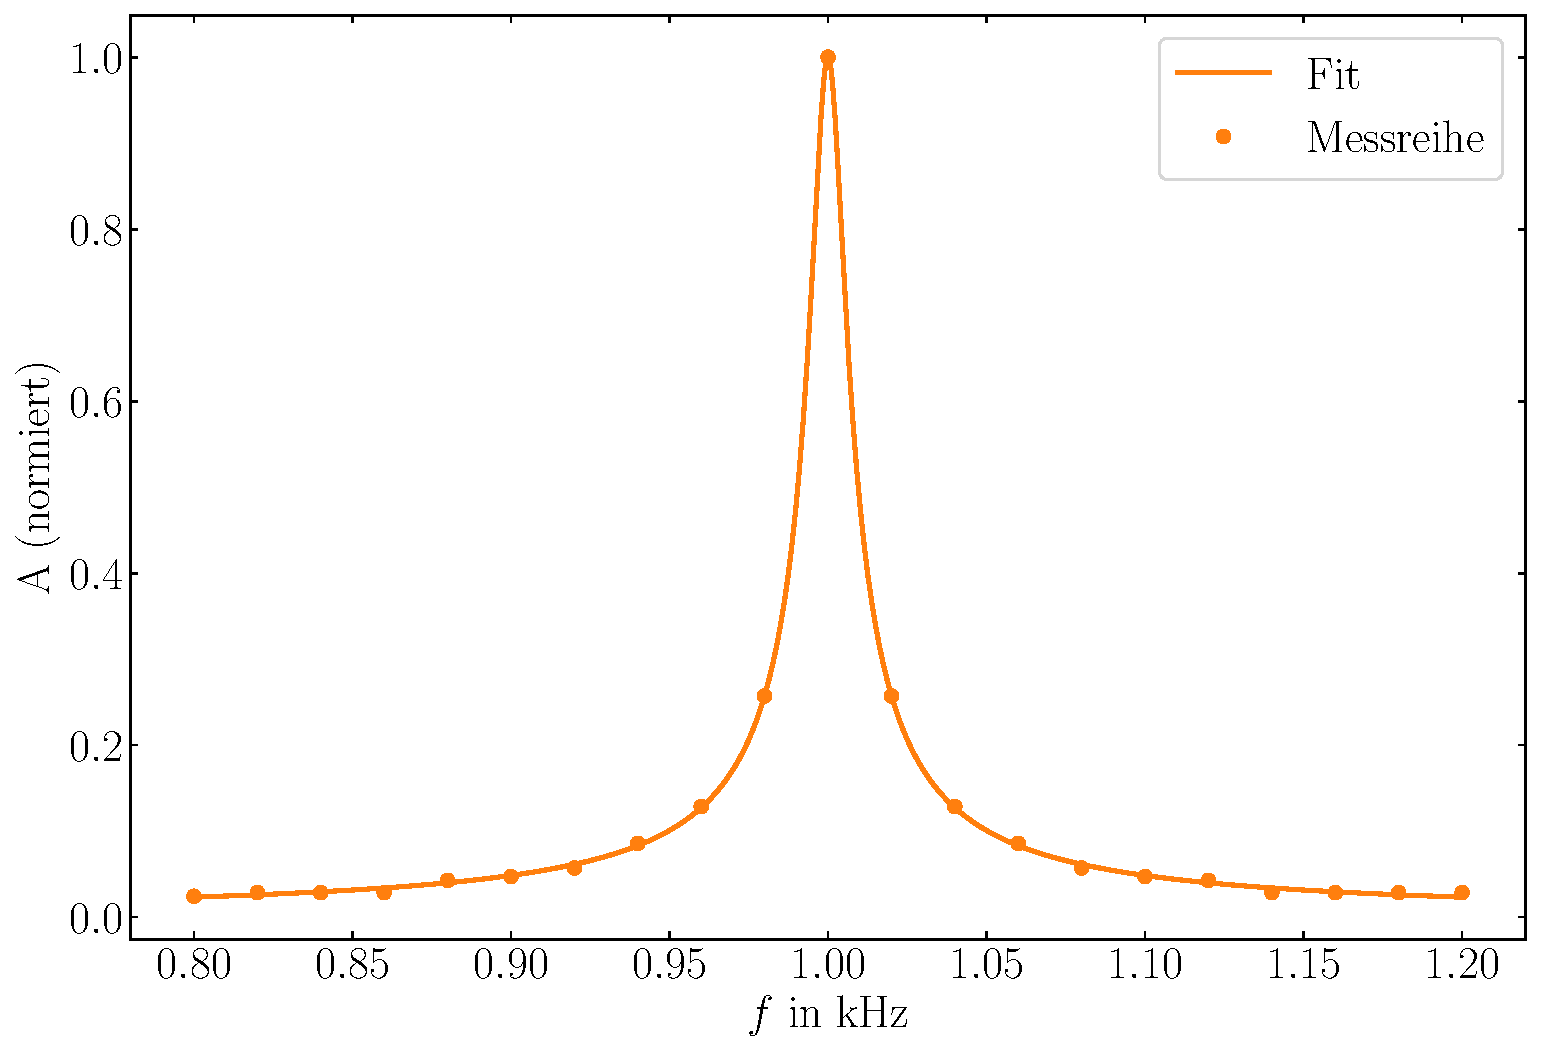
\includegraphics[scale = 0.5]{Manuel/44/6dB.pdf}
    \captionof{figure}{Fit für die Messung mit $\Delta$=6dB}
    \label{image:6dB}
    \vspace{1cm}
    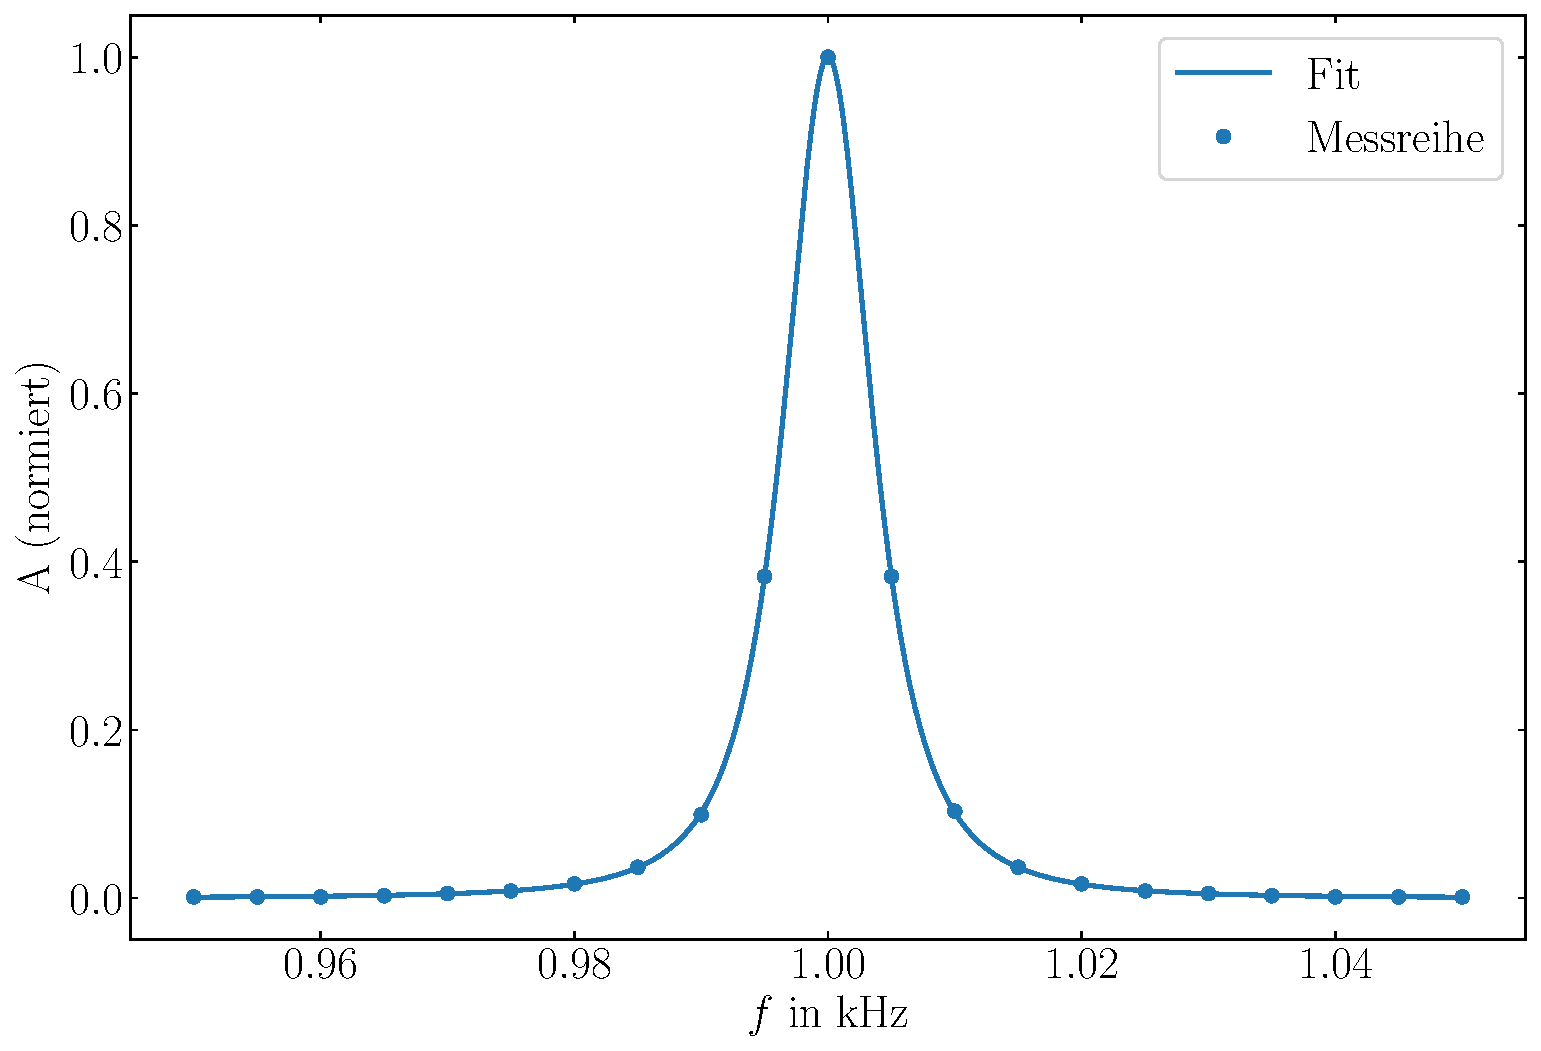
\includegraphics[scale = 0.5]{Manuel/44/18dB.pdf}
    \captionof{figure}{Fit für die Messung mit $\Delta$=18dB}
    \label{image:18dB}
    \vspace{1cm}
    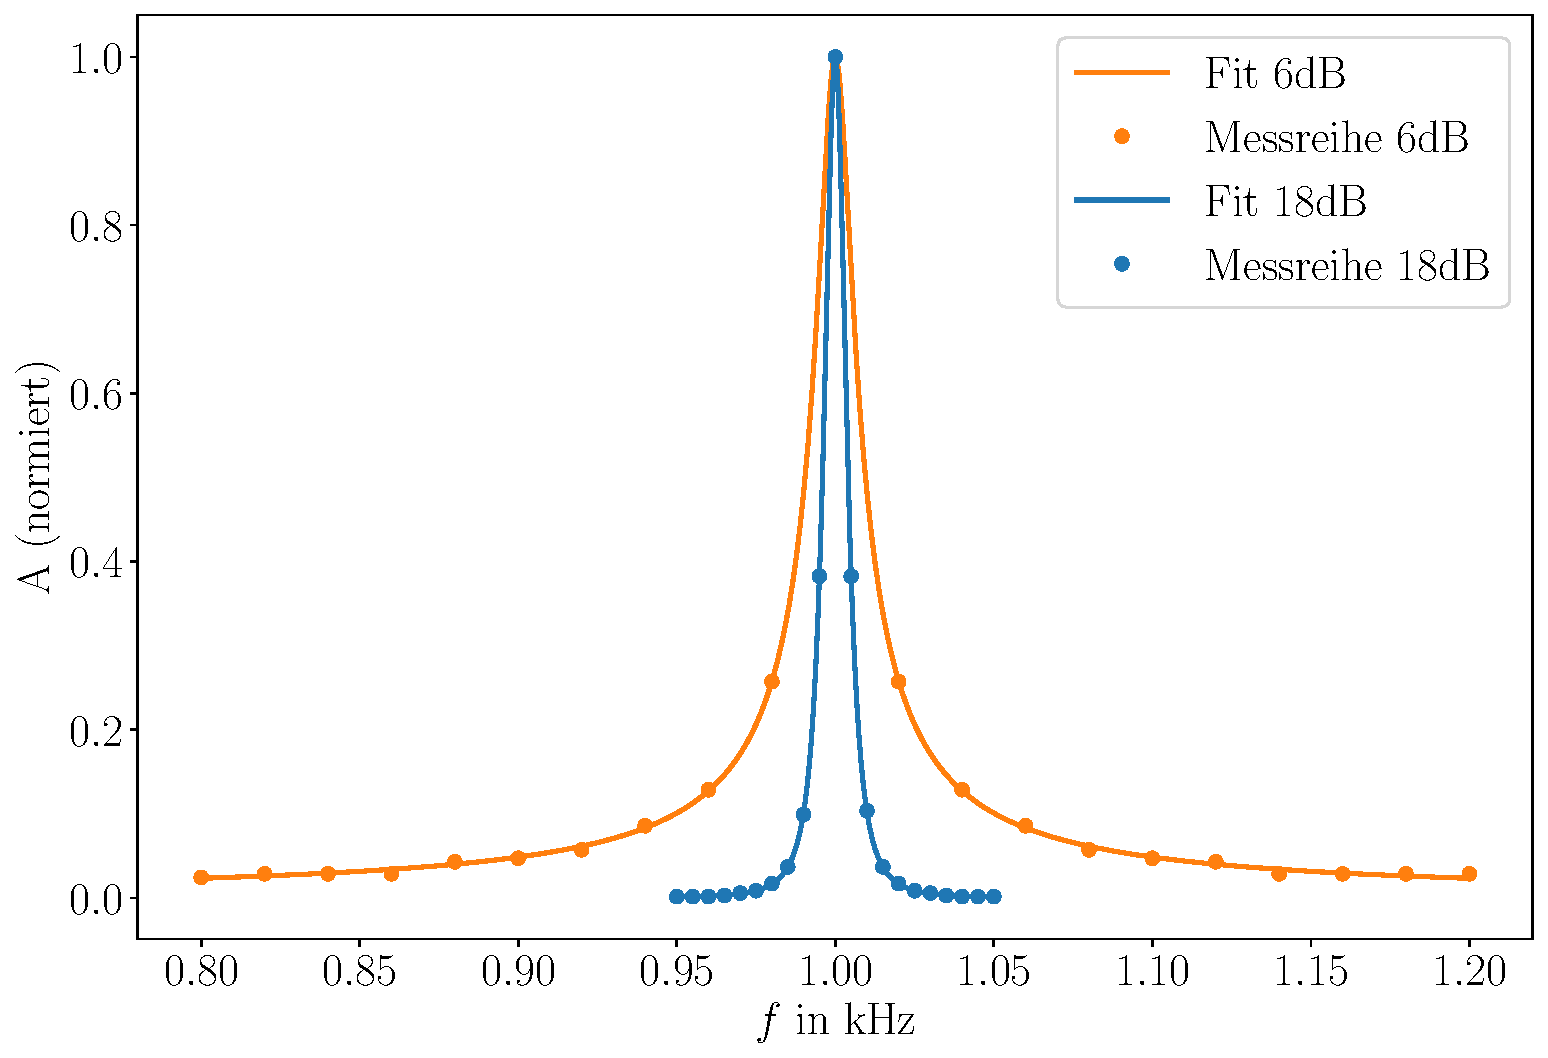
\includegraphics[scale = 0.5]{Manuel/44/All.pdf}
    \captionof{figure}{Vergleich beider Messreihen mit Fit}
    \label{image:All}
\end{center}
\paragraph{c)}\textbf{Lock-In in Praxis}\\
Im letzten Abschnitt wird noch die Verwendung eines Lock-In Verstärkers in der Praxis besprochen. Dazu stand eine Leuchtdiode und eine Photodiode in einer Box mit Deckel zur Verfügung. Die Signale von Leuchtdiode und Photodiode wurden dann auf dem Oszilloskop betrachtet. Man konnte beobachten, dass bei offenen Deckel große Schwankungen am Oszilloskop entstanden. Dies kann damit erklärt werden, das die Photodiode neben dem Signal der Leuchtdiode auch das Licht der Beleuchtung des Raums registriert hat, welches mit 50Hz flackert. Wurde der Deckel geschlossen, ließen die Schwankung nach und die Photodiode detektierte nur noch das Signal der Leuchtdiode, welches trotzdem sehr verrauscht war (zu sehen in Abb. \ref{image:oszi}). 

Die Änderung der Zeitkonstante $\tau$ und Flankensteilheit $\Delta$ am Lock-In Verstärker ergaben eine Veränderung der Auflösung des Lock-In Verstärkers. Dabei war die Auflösung am höchsten, wenn auch die Zeitkonstante und Flankensteilheit am höchsten waren.